\subsection{Slave Jordfugt Implementering}
\label{ch:slave_jordfugt_impl}

Den - ganske simple - HW der syntetiseres i blokken Slave Jordfugt er vist på Figur \ref{fig:topdesign_jordfugt}. 

Der er en \IIC slave komponent, der varetager kommunikationen på \IIC bussen og en analog til digital converter, der læser på de seks jordfugtsensorer. 
Når ADC'en startes, opdaterer den løbende seks registre, uanset hvad PSoC'en ellers laver. 

\begin{figure}[h]
\centering 
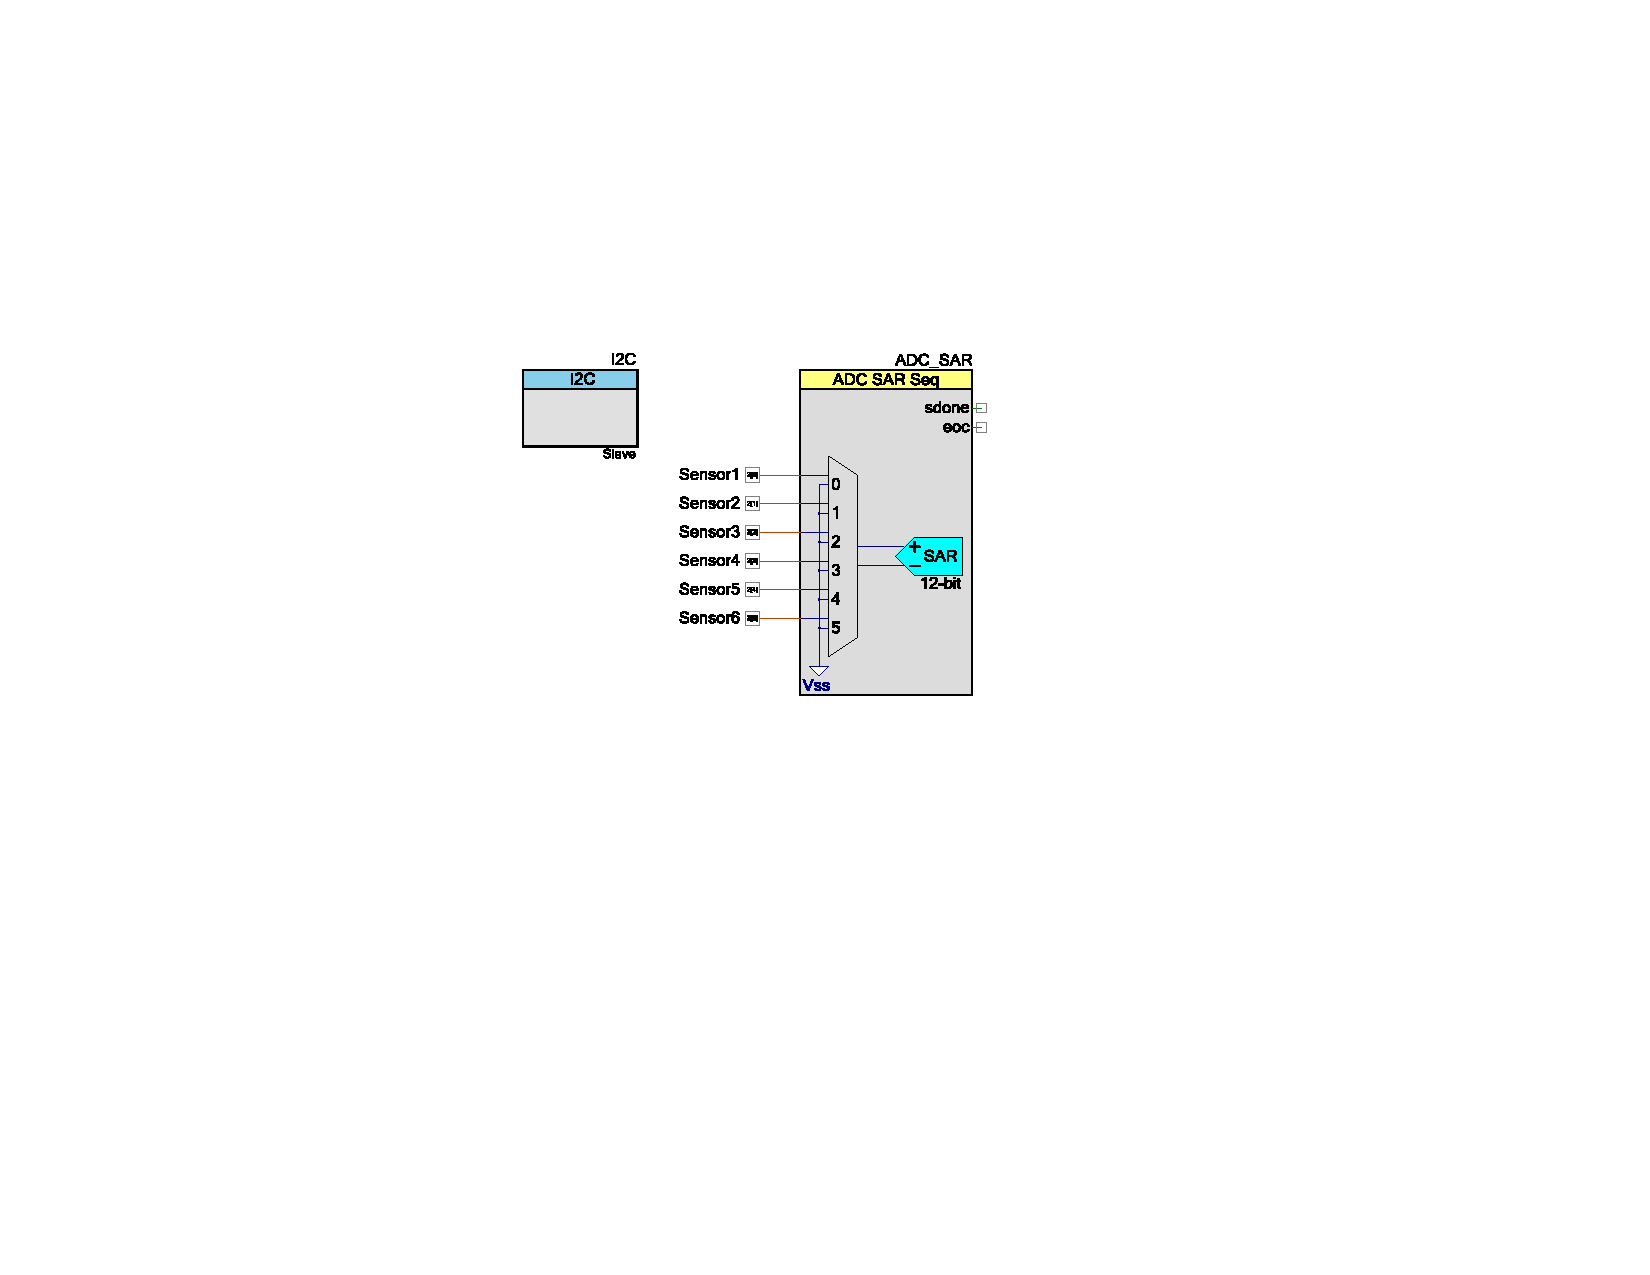
\includegraphics[width={\textwidth-8cm}, trim = 250 270 310 160, clip=true] {../fig/TopDesign_Jordfugt.pdf}
\caption{TopDesign.cysch for PSoC 4 i Jordfugt}
\label{fig:topdesign_jordfugt}
\end{figure}

For detaljeret information om den kode, der afvikles jf. state machinen under design i denne rapport (Figur \ref{fig:stm_jordfugt}, side \pageref{fig:stm_jordfugt}), se afsnit \ref{P-sec:JrdImpl} \nameref{P-sec:JrdImpl} på side \pageref{P-sec:JrdImpl} i projektdokumentationen.